\section{球坐标系下的分离变量法}
\idx{球坐标}{qiuzuobiao}
\idx{勒让德多项式}{lerangde}
\idx{球谐函数}{qiuxie}
\label{sec:spherical}

球坐标里的拉普拉斯算子是\eqref{eq:laplace-sph}.静电、稳态温度和引力势在无源区域都满足 $\nabla^2 u=0$.设
\begin{equation}
  u(r,\theta,\phi)=R(r)\,\Theta(\theta)\,\Phi(\phi),
\end{equation}
代入后乘 $r^2/(R\Theta\Phi)$,
\begin{equation}
  \frac{1}{R}\frac{\mathrm{d}}{\mathrm{d}r}
    \Bigl(r^2\frac{\mathrm{d}R}{\mathrm{d}r}\Bigr)
  =-\frac{1}{\Theta\sin\theta}\frac{\mathrm{d}}{\mathrm{d}\theta}
      \Bigl(\sin\theta\frac{\mathrm{d}\Theta}{\mathrm{d}\theta}\Bigr)
   -\frac{1}{\Phi\sin^2\theta}\frac{\mathrm{d}^2\Phi}{\mathrm{d}\phi^2}.
  \label{eq:sph-separated}
\end{equation}
左边只依赖 $r$.右边再乘 $\sin^2\theta$ 之后,$\phi$ 的部分可以单独分离出来.

\subsection{方位角}
$\Phi(\phi+2\pi)=\Phi(\phi)$,所以
\begin{equation}
  \frac{1}{\Phi}\frac{\mathrm{d}^2\Phi}{\mathrm{d}\phi^2}=-m^2,
  \qquad
  \Phi=e^{\imath m\phi},
  \qquad m\in\mathbb{Z}.
\end{equation}
$m=0$ 是轴对称情形.把 $-m^2$ 代回\eqref{eq:sph-separated},右边变成只含 $\theta$ 的式子,它必须等于常数.为了让极角方程在 $\theta=0,\pi$ 有有限解,这个常数写成 $\ell(\ell+1)$, $\ell=0,1,2,\ldots$,并且 $|m|\leq\ell$.径向方程于是是
\begin{equation}
  \frac{\mathrm{d}}{\mathrm{d}r}
    \Bigl(r^2\frac{\mathrm{d}R}{\mathrm{d}r}\Bigr)
  -\ell(\ell+1)R=0.
  \label{eq:radial-euler}
\end{equation}
试 $R=r^{\alpha}$,得到 $\alpha(\alpha+1)=\ell(\ell+1)$,两个根是 $\alpha=\ell$ 和 $\alpha=-(\ell+1)$.因此
\begin{equation}
  R(r)=A\, r^{\ell}+B\, r^{-(\ell+1)}.
  \label{eq:radial-power}
\end{equation}
含原点的区域丢掉负幂,外部问题在无穷远处丢掉正幂.

若方程是亥姆霍兹方程 $\nabla^2 u+k^2 u=0$,径向因子改成球贝塞尔函数 $j_{\ell}(kr)$,见特殊函数一章.$k=0$ 时幂次解\eqref{eq:radial-power}就是它的极限.

\subsection{勒让德方程}
极角方程是
\begin{equation}
  \frac{1}{\sin\theta}\frac{\mathrm{d}}{\mathrm{d}\theta}
    \Bigl(\sin\theta\frac{\mathrm{d}\Theta}{\mathrm{d}\theta}\Bigr)
  +\Biggl[\ell(\ell+1)-\frac{m^2}{\sin^2\theta}\Biggr]\Theta=0.
  \label{eq:theta-eq}
\end{equation}
令 $x=\cos\theta$,则 $\mathrm{d}/\mathrm{d}\theta=-\sin\theta\,\mathrm{d}/\mathrm{d}x$,并且
\begin{equation}
  \frac{1}{\sin\theta}\frac{\mathrm{d}}{\mathrm{d}\theta}
    \Bigl(\sin\theta\frac{\mathrm{d}\Theta}{\mathrm{d}\theta}\Bigr)
  =\frac{\mathrm{d}}{\mathrm{d}x}
    \Biggl((1-x^2)\frac{\mathrm{d}\Theta}{\mathrm{d}x}\Biggr).
\end{equation}
\eqref{eq:theta-eq}变成连带勒让德方程
\begin{equation}
  (1-x^2)\frac{\mathrm{d}^2 P}{\mathrm{d}x^2}
  -2x\frac{\mathrm{d}P}{\mathrm{d}x}
  +\Biggl[\ell(\ell+1)-\frac{m^2}{1-x^2}\Biggr]P=0,
  \label{eq:associated-legendre}
\end{equation}
其中 $P(x)=\Theta(\arccos x)$,$x\in[-1,1]$.

$m=0$ 时它退化为勒让德方程
\begin{equation}
  (1-x^2)P_{\ell}''-2x P_{\ell}'+\ell(\ell+1)P_{\ell}=0.
  \label{eq:legendre-ode}
\end{equation}
在 $x=\pm 1$ 有限的解是 $\ell$ 次多项式 $P_{\ell}(x)$.级数解在端点一般有对数奇性,只有 $\ell$ 是非负整数时级数截成多项式.

\subsection{罗德里格斯公式}
\begin{equation}
  P_{\ell}(x)
  =\frac{1}{2^{\ell}\ell!}
    \frac{\mathrm{d}^{\ell}}{\mathrm{d}x^{\ell}}(x^2-1)^{\ell}.
  \label{eq:rodrigues}
\end{equation}
$(x^2-1)^{\ell}$ 是 $2\ell$ 次多项式,求导 $\ell$ 次后是 $\ell$ 次多项式,并且 $P_{\ell}(1)=1$.

\begin{figure}[htb]
  \centering
  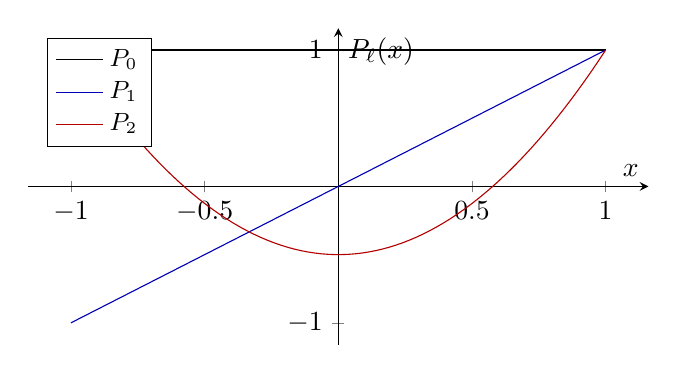
\begin{tikzpicture}
\begin{axis}[
    width=0.78\textwidth,
    height=5.6cm,
    xlabel={$x$},
    ylabel={$P_{\ell}(x)$},
    domain=-1:1,
    samples=80,
    legend pos=north west,
    legend style={font=\small},
    axis lines=middle,
    enlargelimits=0.08,
  ]
  \addplot[black] {1};
  \addplot[blue!70!black] {x};
  \addplot[red!70!black] {0.5*(3*x^2-1)};
  \legend{$P_0$,$P_1$,$P_2$}
\end{axis}
\end{tikzpicture}

  \caption{$P_0$, $P_1$, $P_2$.$P_{\ell}$ 在 $(-1,1)$ 里有 $\ell$ 个零点,并且 $P_{\ell}(1)=1$.}
  \label{fig:legendre}
\end{figure}

\begin{example}
用罗德里格斯公式算 $P_0,P_1,P_2$.
\end{example}
\begin{solution}
$\ell=0$ 时没有求导,$P_0=1$.$\ell=1$,
\begin{equation}
  P_1=\frac{1}{2}\frac{\mathrm{d}}{\mathrm{d}x}(x^2-1)=x.
\end{equation}
$\ell=2$, $(x^2-1)^2=x^4-2x^2+1$,二阶导数是 $12x^2-4$,
\begin{equation}
  P_2=\frac{1}{8}(12x^2-4)=\frac{1}{2}(3x^2-1).
\end{equation}
三者都满足 $P_{\ell}(1)=1$.把 $P_2$ 代入\eqref{eq:legendre-ode}: $P_2'=3x$, $P_2''=3$,
\begin{equation}
  (1-x^2)\cdot 3-2x\cdot 3x+6\cdot\frac{1}{2}(3x^2-1)
  =3-3x^2-6x^2+9x^2-3=0.
\end{equation}
\end{solution}

\subsection{正交性与生成函数}
\eqref{eq:legendre-ode}写成自伴形式
\begin{equation}
  \frac{\mathrm{d}}{\mathrm{d}x}\bigl[(1-x^2)P_{\ell}'\bigr]+\ell(\ell+1)P_{\ell}=0.
\end{equation}
$\ell\neq\ell'$ 时,用 $P_{\ell'}$ 和 $P_{\ell}$ 分别乘对方的方程再相减,从 $-1$ 积到 $1$.左边是
\begin{equation}
  \Bigl[(1-x^2)\bigl(P_{\ell'}P_{\ell}'-P_{\ell}P_{\ell'}'\bigr)\Bigr]_{-1}^{1}=0,
\end{equation}
因为 $1-x^2$ 在端点为零,而勒让德多项式的导数在端点有限.因此
\begin{equation}
  \int_{-1}^{1} P_{\ell}(x)P_{\ell'}(x)\,\mathrm{d}x=0,
  \qquad\ell\neq\ell'.
\end{equation}

生成函数
\begin{equation}
  \frac{1}{\sqrt{1-2xt+t^2}}
  =\sum_{\ell=0}^{\infty} P_{\ell}(x)\, t^{\ell},
  \qquad |t|<1.
  \label{eq:legendre-generating}
\end{equation}
$t=0$ 时左边是 $1$,所以 $P_0=1$.对 $t$ 求导再令 $t=0$,得到 $P_1=x$.把 $x=1$ 代入,左边是 $1/(1-t)=\sum t^{\ell}$,因此每个 $P_{\ell}(1)=1$.

模由生成函数的平方积分定出.令
\begin{equation}
  G(x,t)=\frac{1}{\sqrt{1-2xt+t^2}}.
\end{equation}
正交性使交叉项消失,
\begin{equation}
  \int_{-1}^{1} G(x,t)^2\,\mathrm{d}x
  =\sum_{\ell=0}^{\infty} t^{2\ell}\int_{-1}^{1} P_{\ell}(x)^2\,\mathrm{d}x.
\end{equation}
左边直接积,
\begin{equation}
  \int_{-1}^{1}\frac{\mathrm{d}x}{1-2xt+t^2}
  =\frac{1}{t}\ln\frac{1+t}{1-t}
  =2\sum_{\ell=0}^{\infty}\frac{t^{2\ell}}{2\ell+1}.
\end{equation}
比较 $t^{2\ell}$ 的系数,
\begin{equation}
  \int_{-1}^{1} P_{\ell}(x)^2\,\mathrm{d}x=\frac{2}{2\ell+1}.
  \label{eq:legendre-norm}
\end{equation}
于是 $[-1,1]$ 上的勒让德级数是
\begin{equation}
  f(x)=\sum_{\ell=0}^{\infty} a_{\ell} P_{\ell}(x),
  \qquad
  a_{\ell}=\frac{2\ell+1}{2}\int_{-1}^{1} f(x)P_{\ell}(x)\,\mathrm{d}x.
  \label{eq:legendre-series}
\end{equation}

对\eqref{eq:legendre-generating}作 $\partial/\partial t$,用 $(1-2xt+t^2)\partial G/\partial t=(x-t)G$,比较 $t^{\ell}$ 的系数,得到递推
\begin{equation}
  (\ell+1)P_{\ell+1}(x)=(2\ell+1)x P_{\ell}(x)-\ell P_{\ell-1}(x).
  \label{eq:legendre-recurrence}
\end{equation}
由 $P_0$ 和 $P_1$ 可以逐个写出后面的多项式,不必每次都求导.

\begin{example}
把 $f(x)=x^2$ 展开成勒让德级数.
\end{example}
\begin{solution}
$P_2=\half(3x^2-1)$,所以 $x^2=\tfrac{2}{3}P_2+\tfrac{1}{3}P_0$.用系数公式核对.$a_0=\half\int_{-1}^{1}x^2\,\mathrm{d}x=\tfrac{1}{3}$.
\begin{equation}
  a_2=\frac{5}{2}\int_{-1}^{1} x^2\cdot\frac{3x^2-1}{2}\,\mathrm{d}x
  =\frac{5}{2}\cdot\frac{4}{15}
  =\frac{2}{3}.
\end{equation}
更高阶与 $x^2$ 正交,系数是零.这个展开在球面上就是轴对称势的 $\ell=0$ 和 $\ell=2$ 两项.
\end{solution}

\subsection{连带勒让德函数}
$m\geq 0$ 时,连带勒让德函数由 $P_{\ell}$ 定义,
\begin{equation}
  P_{\ell}^{m}(x)
  =(-1)^{m}(1-x^2)^{m/2}\frac{\mathrm{d}^{m}}{\mathrm{d}x^{m}}P_{\ell}(x).
  \label{eq:assoc-def}
\end{equation}
前面的 $(-1)^{m}$ 是 Condon--Shortley 相位.负阶由
\begin{equation}
  P_{\ell}^{-m}(x)
  =(-1)^{m}\frac{(\ell-m)!}{(\ell+m)!}P_{\ell}^{m}(x)
\end{equation}
定出,这样 $|m|\leq\ell$ 的全部函数都归到 $m\geq 0$ 的导数上.$m>\ell$ 时 $\ell$ 次多项式的 $m$ 阶导数是零.

\begin{example}
$P_2^{1}$ 与 $P_1^{1}$.
\end{example}
\begin{solution}
$P_1=x$,所以 $P_1^{1}=-(1-x^2)^{1/2}=-\sin\theta$.$P_2' =3x$,
\begin{equation}
  P_2^{1}(x)=-3x\sqrt{1-x^2}=-3\cos\theta\sin\theta.
\end{equation}
$x=\pm 1$ 时因子 $\sqrt{1-x^2}$ 是零,极点上 $m\neq 0$ 的连带函数消失,方位角才可以不确定.
\end{solution}

固定 $m$ 时,它们在 $[-1,1]$ 上正交,
\begin{equation}
  \int_{-1}^{1} P_{\ell}^{m}(x)P_{\ell'}^{m}(x)\,\mathrm{d}x
  =\frac{2}{2\ell+1}\frac{(\ell+m)!}{(\ell-m)!}\,\delta_{\ell\ell'}.
  \label{eq:assoc-norm}
\end{equation}
$m=0$ 时回到\eqref{eq:legendre-norm}.同一 $\ell$ 的递推是
\begin{equation}
  (\ell-m+1)P_{\ell+1}^{m}(x)
  =(2\ell+1)x P_{\ell}^{m}(x)
  -(\ell+m)P_{\ell-1}^{m}(x).
\end{equation}

\subsection{球谐函数}
球面上的归一化本征函数是球谐函数
\begin{equation}
  Y_{\ell}^{m}(\theta,\phi)
  =N_{\ell m}\, P_{\ell}^{m}(\cos\theta)\, e^{\imath m\phi},
  \label{eq:spherical-harmonic}
\end{equation}
\begin{equation}
  N_{\ell m}
  =\sqrt{\frac{2\ell+1}{4\pi}\frac{(\ell-m)!}{(\ell+m)!}}.
\end{equation}
相位已经放在\eqref{eq:assoc-def}里,这里不再乘 $(-1)^{m}$.$m<0$ 时把负阶的 $P_{\ell}^{m}$ 代进同一公式.面积元 $\mathrm{d}\Omega=\sin\theta\,\mathrm{d}\theta\,\mathrm{d}\phi$,
\begin{equation}
  \int Y_{\ell}^{m}\,\overline{Y_{\ell'}^{m'}}\,\mathrm{d}\Omega
  =\delta_{\ell\ell'}\delta_{mm'}.
\end{equation}
前几个是
\begin{align}
  Y_0^{0}&=\frac{1}{\sqrt{4\pi}}, \\
  Y_1^{0}&=\sqrt{\frac{3}{4\pi}}\cos\theta, \\
  Y_1^{\pm 1}&=\mp\sqrt{\frac{3}{8\pi}}\sin\theta\, e^{\pm\imath\phi}.
\end{align}
$Y_1^{0}$ 的归一化可以手算:方位角积出 $2\pi$,再令 $u=\cos\theta$,
\begin{equation}
  \int |Y_1^{0}|^2\,\mathrm{d}\Omega
  =\frac{3}{4\pi}\cdot 2\pi\int_{-1}^{1} u^2\,\mathrm{d}u
  =\frac{3}{2}\cdot\frac{2}{3}=1.
\end{equation}

球面上的函数展开成
\begin{equation}
  F(\theta,\phi)
  =\sum_{\ell=0}^{\infty}\sum_{m=-\ell}^{\ell}
    c_{\ell m} Y_{\ell}^{m}(\theta,\phi),
  \qquad
  c_{\ell m}=\int F\,\overline{Y_{\ell}^{m}}\,\mathrm{d}\Omega.
\end{equation}
轴对称时只剩 $m=0$,而 $Y_{\ell}^{0}$ 正比于 $P_{\ell}(\cos\theta)$,展开就是\eqref{eq:legendre-series}.

\subsection{均匀电场中的导体球}

\begin{figure}[htb]
  \centering
  \begin{tikzpicture}[font=\small, >=Stealth,
    vec/.style={-{Stealth[length=2mm]}, line width=0.7pt}]
  \draw[gray!35, thin] (0,-2.15) -- (0,2.35) node[above] {$z$};
  \draw[gray!35, thin] (-2.2,0) -- (2.2,0) node[right] {$x$};
  \fill[blue!8] (0,0) circle (0.9);
  \draw[blue!70!black, thick] (0,0) circle (0.9);
  \foreach \x in {-1.2,-0.4,0.4,1.2} {
    \draw[vec, gray!75] (\x,-2.05) -- (\x,-1.15);
    \draw[vec, gray!75] (\x,1.15) -- (\x,2.05);
  }
  \draw[vec, red!70!black] (0,0.9) -- (0,1.7) node[midway, right] {$3E_0$};
  \draw[vec, red!70!black] (0,-1.7) -- (0,-0.9);
  \node at (0,0) {导体};
  \node[font=\scriptsize, gray] at (1.55,1.85) {$\mathbf{E}_0$};
\end{tikzpicture}

  \caption{均匀电场中的中性导体球.极点上的法向场是 $3E_0$,赤道上法向场为零.}
  \label{fig:sphere-field}
\end{figure}

半径为 $a$ 的导体球放在沿 $z$ 轴的均匀电场 $\mathbf{E}_0$ 里,球面电位取为零.球外 $\nabla^2 V=0$,轴对称,所以
\begin{equation}
  V(r,\theta)
  =\sum_{\ell=0}^{\infty}
    \bigl(A_{\ell} r^{\ell}+B_{\ell} r^{-(\ell+1)}\bigr) P_{\ell}(\cos\theta).
\end{equation}
远处 $V\sim -E_0 z=-E_0 r\cos\theta=-E_0 r P_1(\cos\theta)$,因此 $A_1=-E_0$,其余 $A_{\ell}=0$.负幂在无穷远处自己消失,可以保留.球面 $V(a,\theta)=0$ 要求每一项的两个径向系数抵消,
\begin{equation}
  B_1=-A_1 a^{3}=E_0 a^{3},
\end{equation}
其它 $B_{\ell}=0$.于是
\begin{equation}
  V(r,\theta)
  =-E_0\Bigl(r-\frac{a^3}{r^2}\Bigr)\cos\theta,
  \qquad r\geq a.
  \label{eq:sphere-potential}
\end{equation}

\begin{example}
球面上的电场,以及它和圆柱结果的差别.
\end{example}
\begin{solution}
\begin{equation}
  E_r=-\frac{\partial V}{\partial r}
  =E_0\Bigl(1+\frac{2a^3}{r^3}\Bigr)\cos\theta.
\end{equation}
$r=a$ 时 $E_r=3E_0\cos\theta$.两极是 $3E_0$,不是圆柱表面上的 $2E_0$.赤道 $\theta=\pi/2$ 上 $\cos\theta=0$,法向场为零.$r=a$ 时括号 $r-a^3/r^2$ 是零,球面保持零势.感应面电荷 $\sigma=\varepsilon_0 E_r=3\varepsilon_0 E_0\cos\theta$,北半球与南半球反号,总电荷是零.
\end{solution}

\subsection{球面上给定的电位}

\begin{example}
球内势在原点有限,球面电位是 $V(a,\theta)=V_0\cos\theta$.
\end{example}
\begin{solution}
内部丢掉 $r^{-(\ell+1)}$.边界是 $P_1$,只留下
\begin{equation}
  V(r,\theta)=A_1 r\cos\theta,
  \qquad A_1 a=V_0,
\end{equation}
\begin{equation}
  V(r,\theta)=V_0\frac{r}{a}\cos\theta=V_0\frac{z}{a}.
\end{equation}
球外、无穷远处趋于零的对应问题丢掉 $r^{\ell}$,
\begin{equation}
  V(r,\theta)=V_0\frac{a^2}{r^2}\cos\theta,
  \qquad r\geq a.
\end{equation}
一般的轴对称球面电位 $f(\theta)$ 先按 $x=\cos\theta$ 作勒让德展开,$a_{\ell}$ 用\eqref{eq:legendre-series}.球内是 $\sum a_{\ell}(r/a)^{\ell} P_{\ell}(\cos\theta)$,球外是 $\sum a_{\ell}(a/r)^{\ell+1} P_{\ell}(\cos\theta)$.
\end{solution}
